\documentclass[8pt]{beamer}
\usepackage[utf8]{inputenc}
\usepackage{xcolor}
\usepackage{graphicx}
\usepackage{colortbl}
\usepackage{epsfig}
% \usepackage{cancel}
\usepackage{ulem}
% \usepackage{threeparttable} % Joao Pela: 
\usepackage{amsmath}
\usepackage{hyperref}
\usepackage{appendixnumberbeamer}
\usepackage{feynmp}         % For latex produced Feynman Diagrams
\usepackage{pgfgantt}

\newcommand\Fontvi{\fontsize{6}{7.2}\selectfont}

\newcommand{\totlumi}{19.6~fb$^{-1}$}
\newcommand{\pta}{p_{\rm T}^{\rm j1}}
\newcommand{\ptb}{p_{\rm T}^{\rm j2}}
\newcommand{\etaa}{\eta_{\rm j1}}
\newcommand{\etab}{\eta_{\rm j2}}
\newcommand{\sgneta}{\etaa \cdot \etab}
\newcommand{\etajj}{\Delta \eta_{\rm jj}}
\newcommand{\phijj}{\Delta \phi_{\rm jj}}
\newcommand{\mjj}{M_{\rm jj}}
\newcommand{\met}{\displaystyle{\not} E_{\rm T}}
\newcommand{\W}{{\rm W}}
\newcommand{\Z}{{\rm Z}}
\newcommand{\stat}{\text{ (stat.)}}
\newcommand{\syst}{\text{ (syst.)}}

\usetheme{Madrid}

\author[J. Pela]{João Pela, on behalf of the CMS Collaboration}
\title[Search for VBF Higgs $\rightarrow$ Inv at CMS]{Search for invisible Higgs decays in the VBF channel using the CMS detector}
\institute[ICL]{Imperial College London}
\date{2014-04-08}

% The log drawn in the upper right corner.
\logo{\includegraphics[height=0.115\paperheight]{img/Logo_CMSICL.png}}

\begin{document}
\setlength{\unitlength}{1mm}

% ###################################################
\begin{frame}
  \titlepage
\end{frame}

% ###################################################
\begin{frame}{Introduction}
\Fontvi
 
\begin{block}{SM Higgs boson compatibility}
 
All measurements of the 125 GeV boson to date are compatible with a SM Higgs boson, but:
\begin{itemize}
 \item Associated uncertainties are large.
 \item Possibility for non-SM properties remains.
\end{itemize}

Additional SM-like Higgs bosons have been excluded over a wide mass range, additional Higgs bosons with exotic decay modes remains a possibility, and are predicted by many models.

\end{block}

\begin{block}{BSM invisible Higgs boson decay modes:}

\begin{itemize}
 \item Neutralinos in supersymmetric models.
 \item Graviscalars in models with extra dimensions. 
\end{itemize}

\end{block}

\begin{block}{Indirect measurements}

The ATLAS and CMS collaborations have used the visible decay modes to infer limits on the invisible branching fraction of the 125 GeV Higgs boson:
\begin{itemize}
 \item ATLAS: upper limit of 60\% (ATLAS-CONF-2013-034) 
 \item CMS: upper limit of 64\% (CMS-PAS-HIG-13-005)
\end{itemize}

\end{block}

\begin{block}{Motivations for direct searches for invisible decays:}

\begin{itemize}
 \item Observation of a signal in such searches would be a \uline{clear indication} of physics beyond the SM.
 \item Non-observation provides the opportunity to further \uline{constrain the properties} of the newly discovered boson.
\end{itemize}

\end{block}
 
\end{frame}

% ###################################################
\begin{frame}{VBF Channel}

\begin{columns}
 
\column[t]{0.45\linewidth}
\begin{block}{Direct searches channels}

Direct searches rely on associated production modes, where the Higgs recoils against a visible system.
\begin{itemize}
 \item Z Associated production: Low production cross section; Clear final state, but low sensitivity with the available data.
 \item VBF mode: Substantially higher cross section. Shown to offer greater sensitivity to invisible decays.
\end{itemize}

\end{block}

\begin{block}{VBF Higgs Diagram}
 
\centering
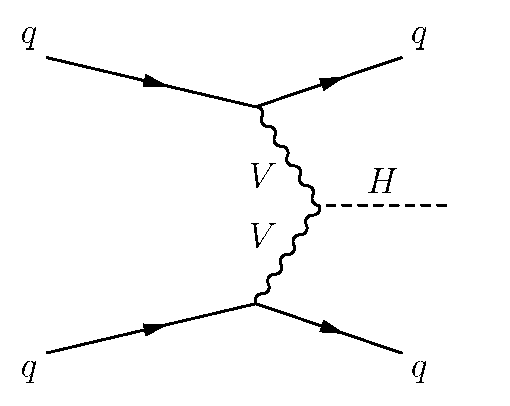
\includegraphics[width=0.45\linewidth]{img/feyn_VBF.pdf} 

\end{block}

\column[t]{0.45\linewidth}
\begin{block}{VBF Higgs to invisible search}

Search for final states with:
\begin{itemize}
 \item Two separated jets and large missing energy.
 \item Use the distinct topology of the VBF jets to distinguish invisible Higgs decays from background.
\end{itemize}
 
\end{block}

\begin{block}{Backgrounds}

Major:
\begin{itemize}
 \item $\Z \rightarrow \nu \nu$, in association with jets
 \item $\W \rightarrow \ell \nu$, with charged lepton misidentified
\end{itemize}

Minor:
\begin{itemize}
 \item Mismeasured QCD events
 \item Other SM processes ($\W\W,\Z\Z,t\bar{t}, etc.$)
\end{itemize}

\end{block}

\end{columns}

\end{frame}

% ###################################################
\begin{frame}{Analysis Definition}
 
\begin{block}{Dedicated trigger}
 
Requirements:
\begin{itemize}
 \item Any forward/backward pair of jets satisfying:
 \begin{itemize}
  \item Jet $p_t>40 GeV$
  \item $\Delta\eta_{jj} = | \eta_{jet1} - \eta_{jet2}| > 3.5$
  \item High invariant mass ($m_{jj}>800$ GeV)
 \end{itemize}
 \item $\met(\text{no }\mu)>65$ GeV
\end{itemize}
 
\end{block}

\begin{block}{Offline selection}
 
\begin{itemize}
 \item Filter mismeasured MET: remove anomalous calorimeter signals, beam halo, calorimeter laser calibration events and tracking failure. 
 \item Good vertex: ($|z|<24$ cm, $r<2$ cm) and $10+$ tracks
 \item Lepton veto: electron or muon with $p_t>10$ GeV
 
 \item Dijet: leading Particle Flow AK5 jet pair that pass pile-up jet rejection:
 \begin{itemize}
  \item $\eta_{jet1} . \eta_{jet2} < 0$
  \item Jet $p_t > 50$ GeV and $\eta < 4.7$
  \item $m_{jj}>1100$ GeV
  \item $\Delta\phi_{jj} < 1.0$
 \end{itemize}

 \item $PF_{MET} > 130$ GeV
 
 \item Central Jet Veto (CJV): Veto events with any jet where $\eta_{jet1} < \eta_{j} < \eta_{jet2}$ and $p_t>30$ GeV
 
\end{itemize}
 
 
\end{block}
 
\end{frame}

% ###################################################
\begin{frame}{Background Estimation Methods I}
\Fontvi 

\begin{block}
 
We use data control regions and MC control to signal region ratios to extrapolate each major background contribution our signal region. For both $\Z$ and $\W$ background we use $\met(\text{no }\mu)$.

\end{block}

\begin{columns}  
\column[t]{0.65\linewidth}
\begin{block}{$\Z (\rightarrow \nu \nu)+$jets}


\begin{itemize}
 \item Estimated from data using observable $\Z \rightarrow \mu \mu$ decays:
 \item Identical selection for signal region except lepton veto is replaced with a $\Z \rightarrow \mu \mu$ requirement:
 \begin{itemize}
  \item {\Fontvi Require two muons with $p_t > 20 $ GeV, and $60 < M_{\mu\mu}<120$ GeV, Veto on additional leptons.}
 \end{itemize}
\end{itemize}

\end{block}

\begin{block}{$\W (\rightarrow \ell \nu)+$jets}

For $\W \rightarrow {\rm e} \nu$ and $\W \rightarrow \mu \nu$ 
\begin{itemize}
 \item Similar method as $\Z (\rightarrow \nu \nu)+$jets.
 \begin{itemize}
  \item {\Fontvi  Require one reconstructed ${\rm e}/\mu$ with $p_t > 20/10 $ GeV, and $|\eta| < 2.4/2.1$ GeV. Veto additional leptons.}
 \end{itemize}
 \item Presence of $\W$ electron found to be negligible.
\end{itemize}

For $\W \rightarrow \tau\nu$ where the tau decays hadronically
\begin{itemize}
 \item Control region is defined in the same way as $\W \rightarrow \ell \nu$
 \item Require one hadronic tau, no additional leptons
 \item The central jet veto is not applied in order to increase the yield
\end{itemize}

\end{block} 
 
\column[t]{0.32\linewidth}
\begin{block}{$\Z \rightarrow \nu \nu$ mass}

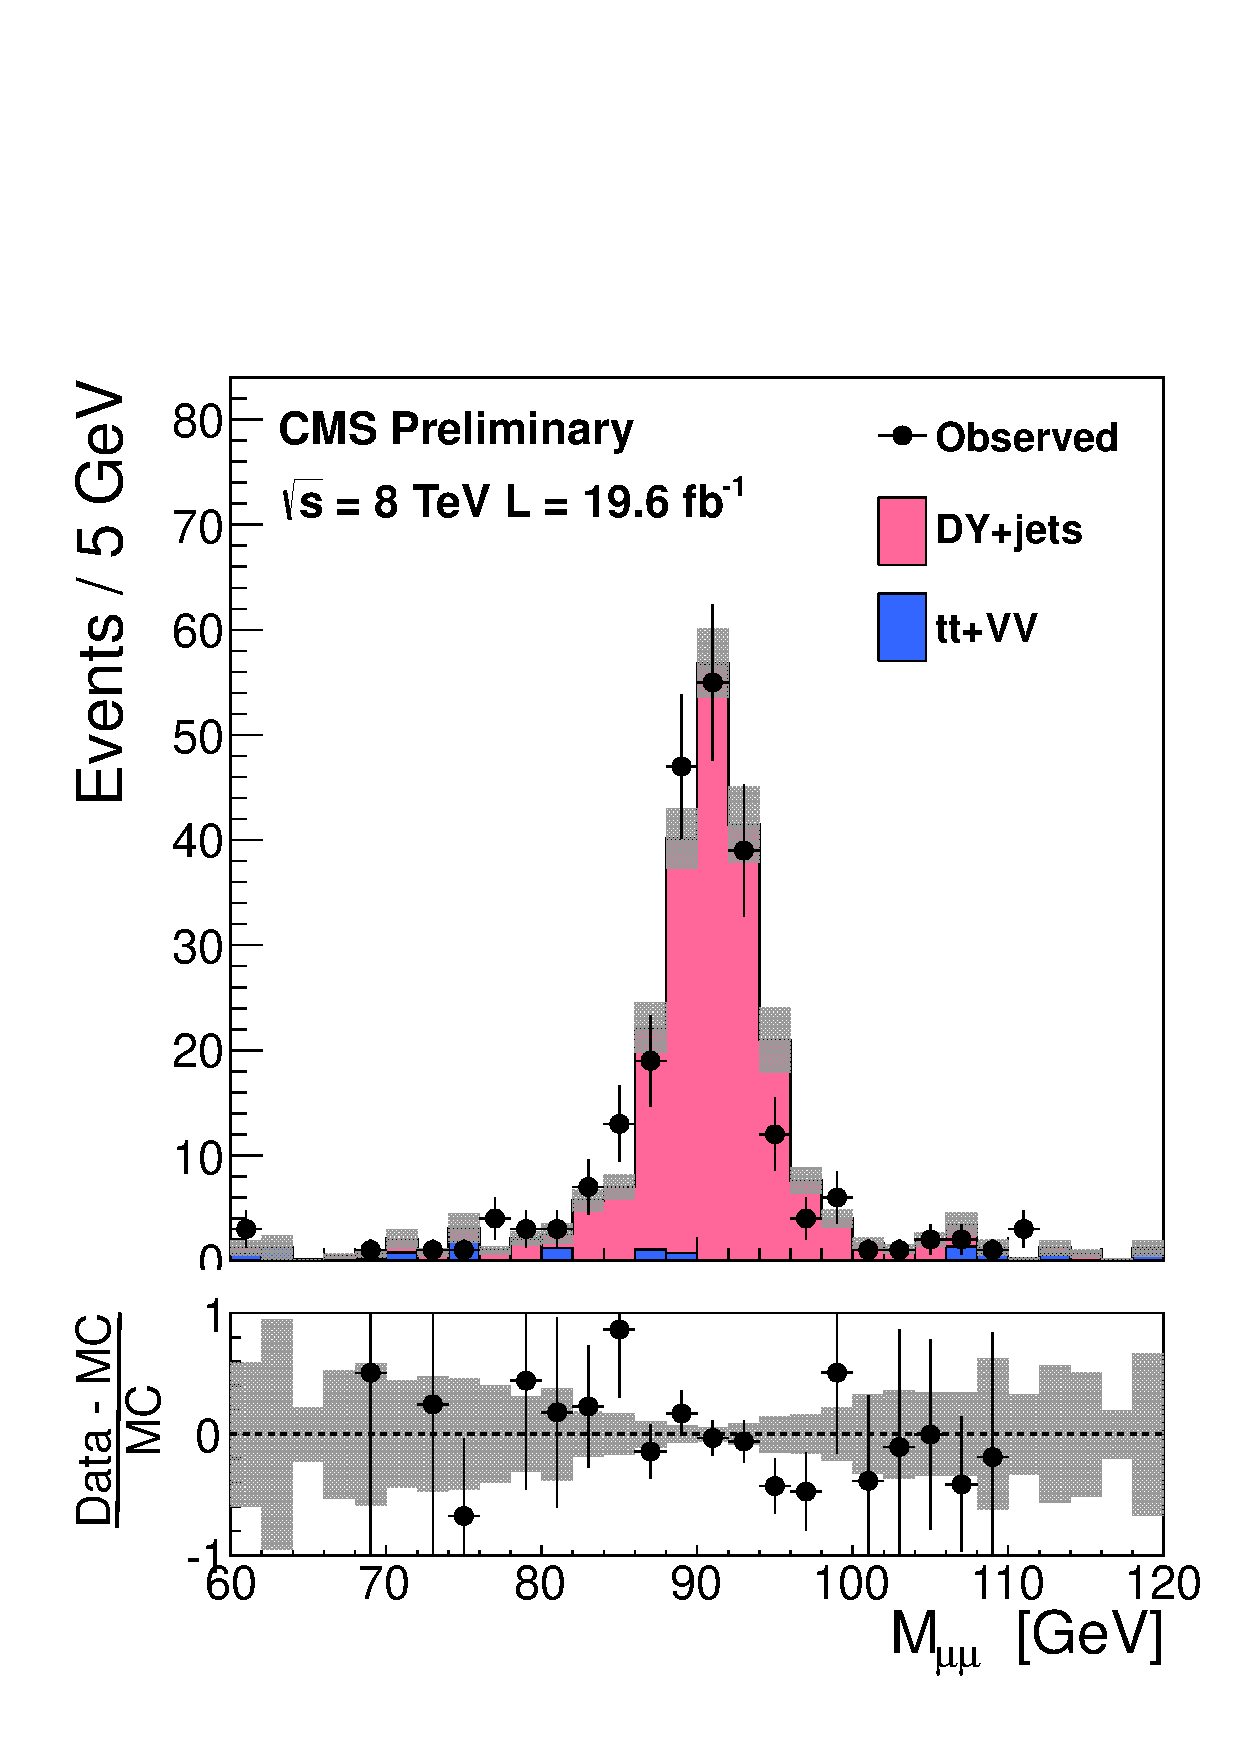
\includegraphics[width=\linewidth]{img/ZCtrlZMass}

\end{block}

\end{columns}
 
\end{frame}

% ###################################################
\begin{frame}{Background Estimation Methods II}

\begin{block}{QCD Multijets}

Use the fractions of events passing the $\met$ and CJV cuts, after the full remaining selection. We define regions ABCD as follows:

\begin{itemize}
 \item{A : fail $\met$, fail CJV}
 \item{B : pass $\met$, fail CJV}
 \item{C : fail $\met$, pass CJV}
 \item{D : pass $\met$, pass CJV}
\end{itemize}

We estimate the QCD multijet component in regions A,B and C by subtracting MC electroweak backgrounds from data. We then estimate the QCD multijet component in the signal region D, to be $N_{D} = N_{B}N_{C} / N_{A}$.

\end{block}

\begin{block}{Other backgrounds}
 
All other minor backgrounds are estimated from MC.
 
\end{block}
 
\end{frame}

% ###################################################
\begin{frame}{Event Yield and Background Estimation}

The signal yield is given for a 125 GeV Higgs with 100\% invisible branching fraction, produced via VBF with the SM production cross section.

\begin{block}{Yields}

\begin{table}[th!]
\centering
% \caption{Summary of estimated backgrounds and observed yield in the signal region.}
\begin{tabular}{|l|c|}
\hline
Background 	 		& $N_{\rm est}$ \\
\hline
$Z \rightarrow \nu\nu$ 		& $102 \pm 30 \stat \pm 26 \syst$	\\
$W \rightarrow \mu\nu$ 	 	& $67.2 \pm 5.0 \stat \pm 15.1 \syst$ 	\\
$W \rightarrow {\rm e} \nu$  	& $68.2 \pm 9.2 \stat \pm 18.1 \syst$	\\
$W \rightarrow \tau \nu$ 	& $54 \pm 16 \stat \pm 18 \syst$ \\
QCD multijet 	 		& $36.8 \pm 5.6 \stat \pm 30.6 \syst$ \\
Other SM			& $10.4 \pm 3.1 \syst$ \\
\hline
Total background		& $339 \pm 36 \stat \pm 50 \syst$  \\
VBF H(inv)                      & $208$ \\
Observed 			& $390$  \\	
\hline
\end{tabular}
\end{table}

\end{block}

In the signal region in data, we observe 390 events, which is \uline{compatible with the background prediction} within 1 $\sigma$.

\end{frame}

% ###################################################
\begin{frame}{Limits on invisible Higgs}
 
We can place upper limit on an invisible Higgs signal.  
\begin{itemize}
 \item Calculated to 95\% C.L. with an asymptotic ${\rm CL}_{\rm S}$ method
 \item Using the standard CMS Higgs combination software package 
\end{itemize}
 
\begin{columns}
 
\column[t]{0.45\linewidth}
\begin{block}
 
\centering
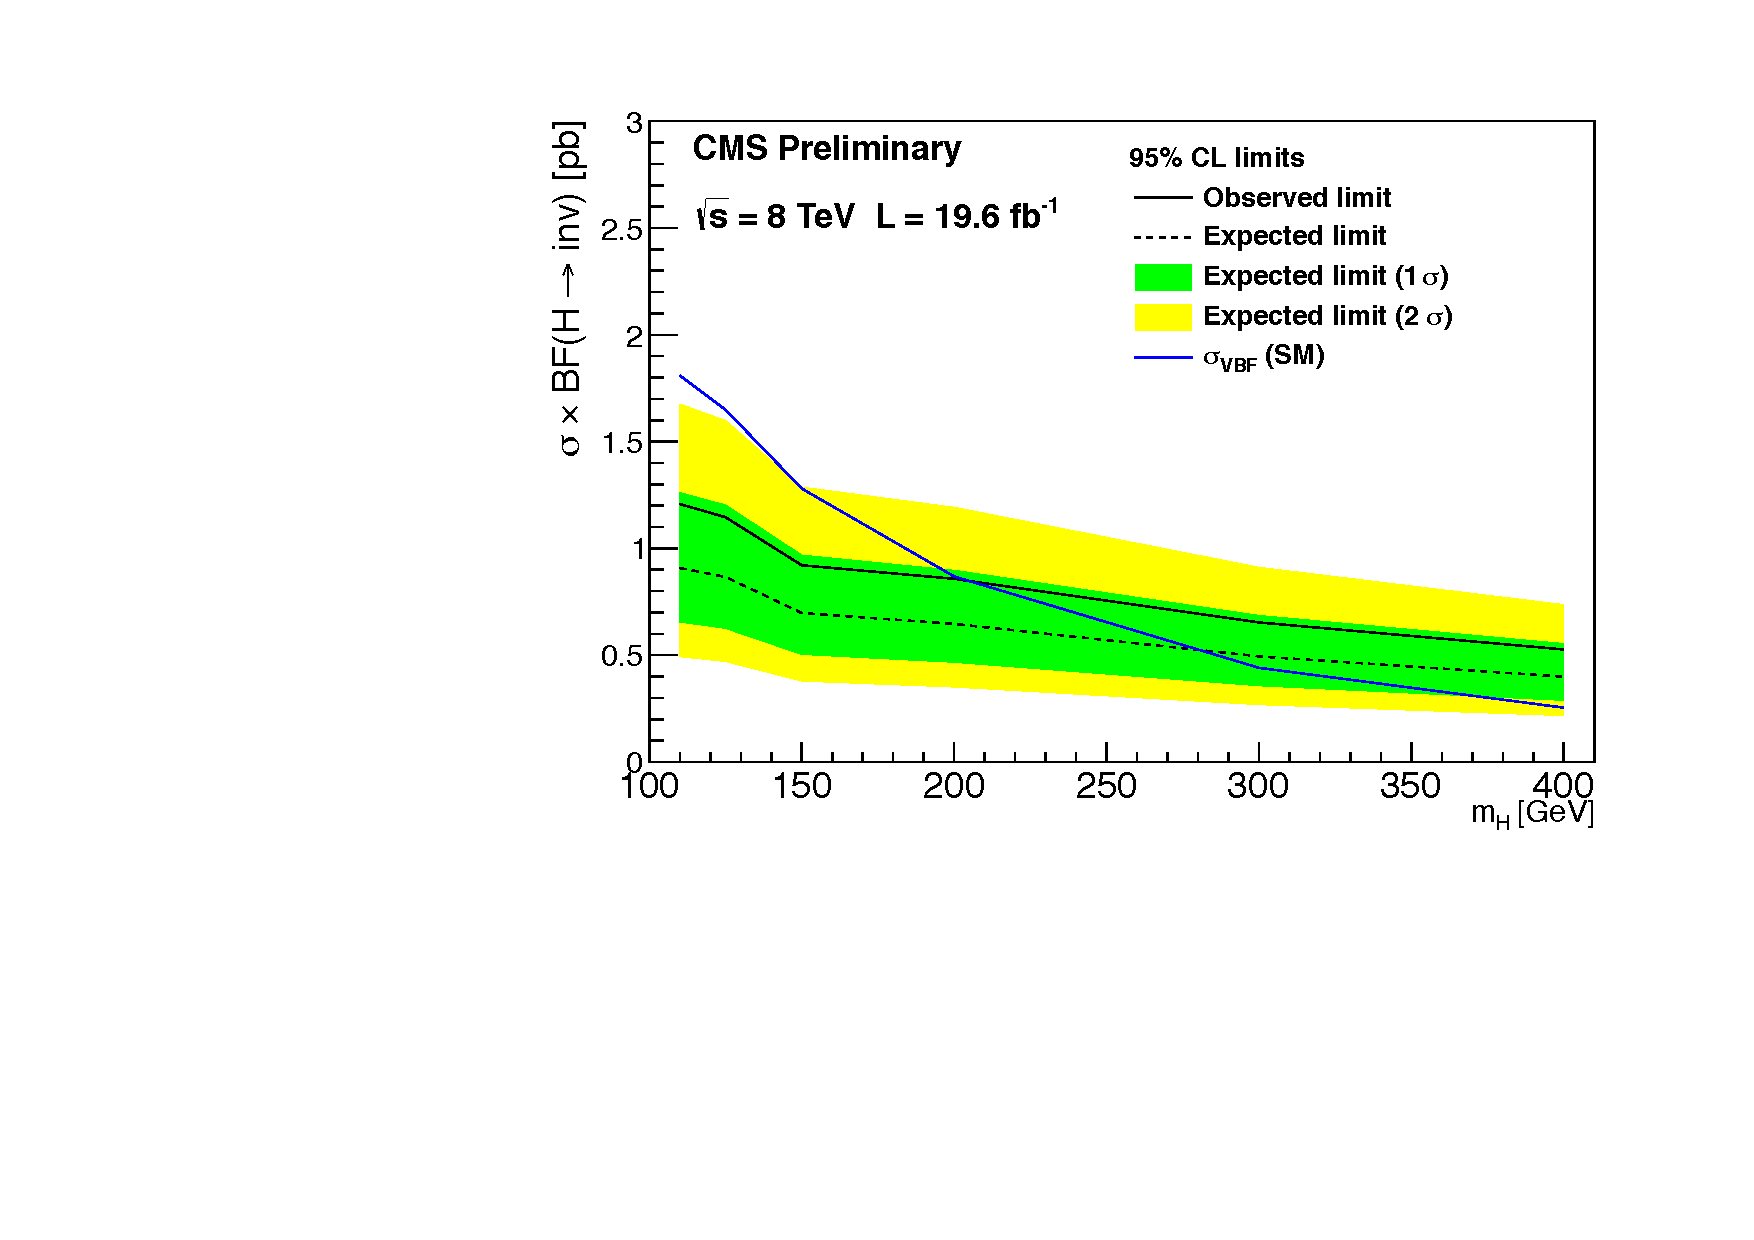
\includegraphics[width=\linewidth]{img/XSLimit.pdf} 

\end{block}

\column[t]{0.45\linewidth}
\begin{block}
 
\centering
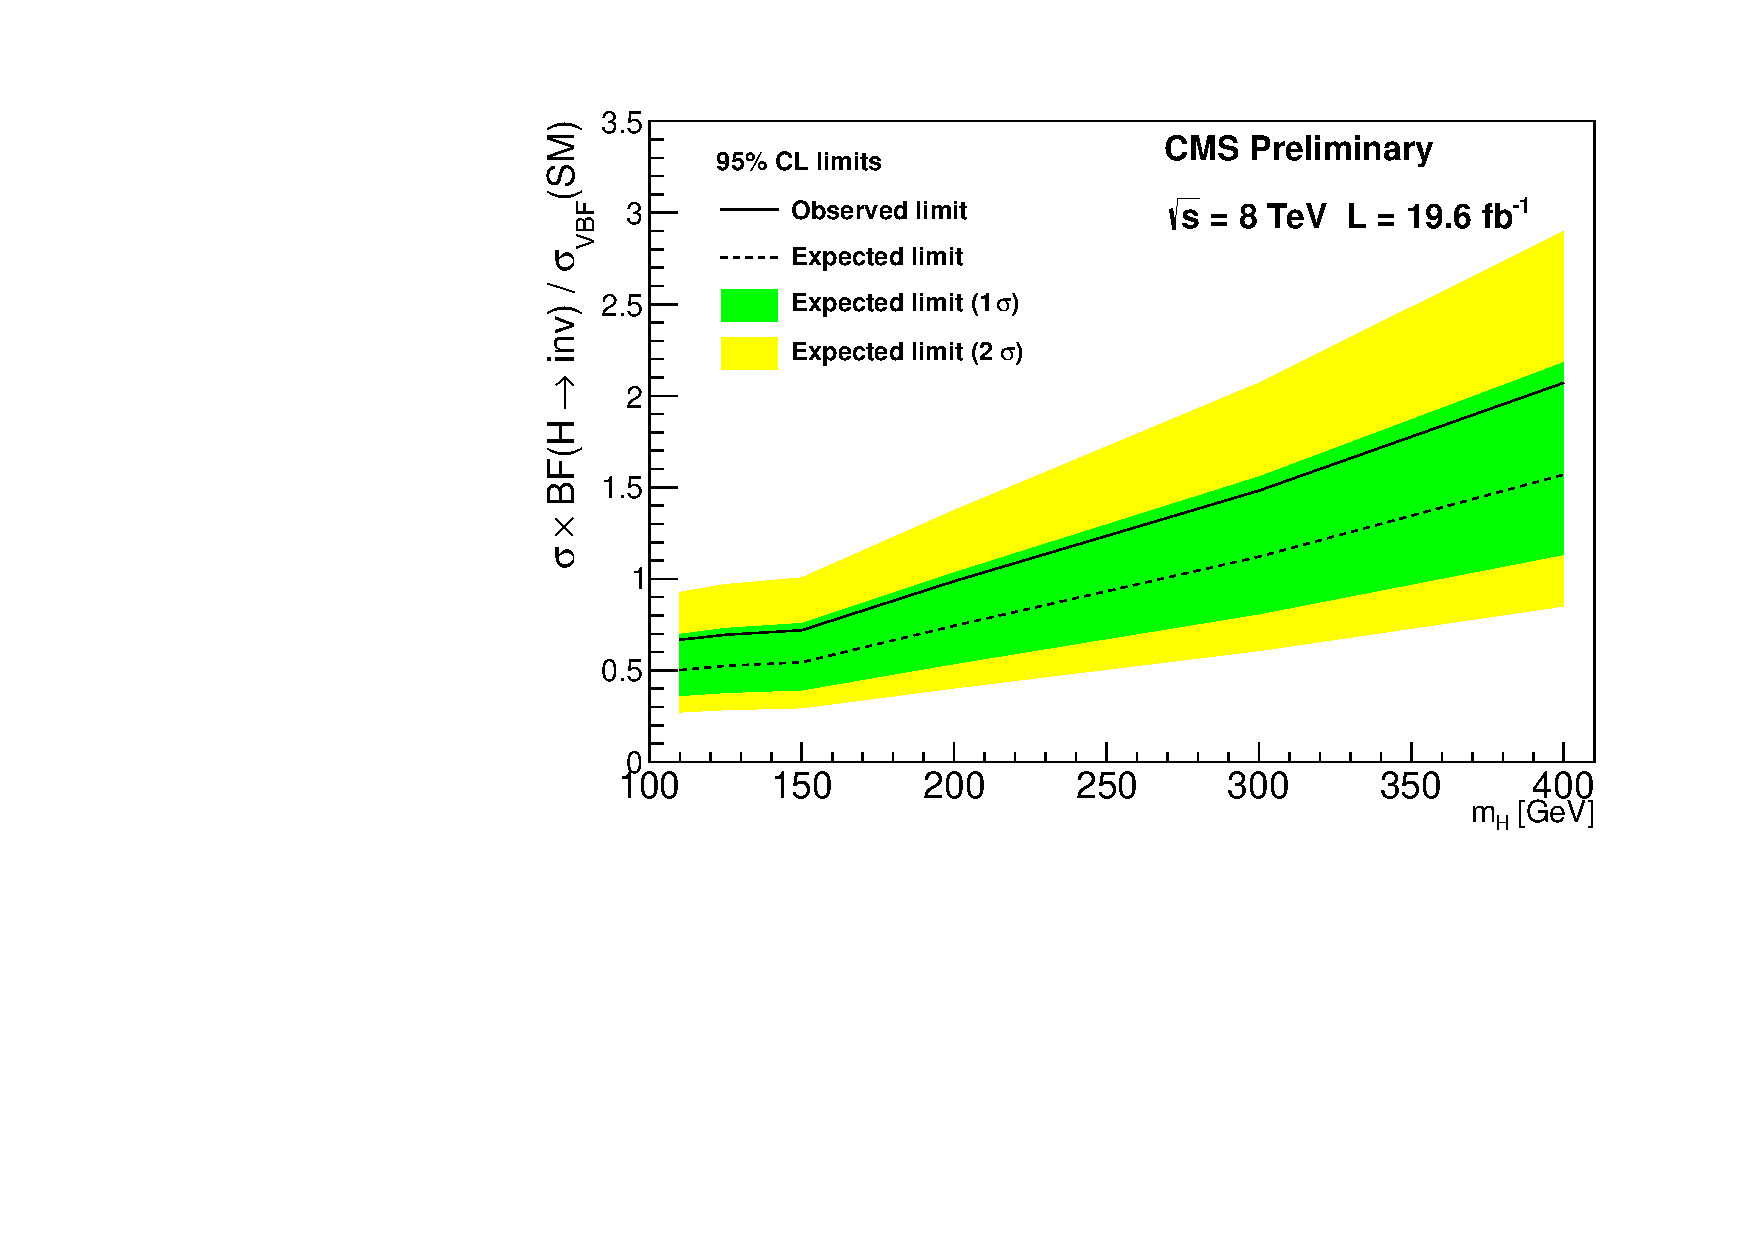
\includegraphics[width=\linewidth]{img/xsiLimit.pdf} 

\end{block}

\end{columns}

\begin{itemize}
 \item On the left, observed and expected limits on the production cross section times invisible branching fraction as a function of the Higgs mass. 
 \item On the right, the same limits, normalised to the SM VBF production cross section.
\end{itemize}

Assuming the SM VBF production cross section, the observed (expected) limit on the \\ invisible branching fraction of the 125 GeV Higgs is 69 (53)\%. 

\end{frame}

% ###################################################
\begin{frame}{Combining VBF H and ZH}
 
Our results were combined with the ones from $ZH, (Z \rightarrow \ell\ell)$  analysis to obtain further sensitivity.
 
\begin{columns}
 
\column[t]{0.45\linewidth}
\begin{block}{VBF Higgs Diagram}
 
\centering
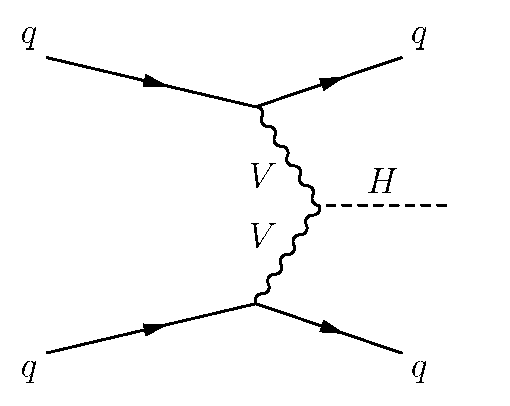
\includegraphics[width=0.8\linewidth]{img/feyn_VBF.pdf} 

\end{block}

\column[t]{0.45\linewidth}
\begin{block}{ZH Diagram}
 
\centering
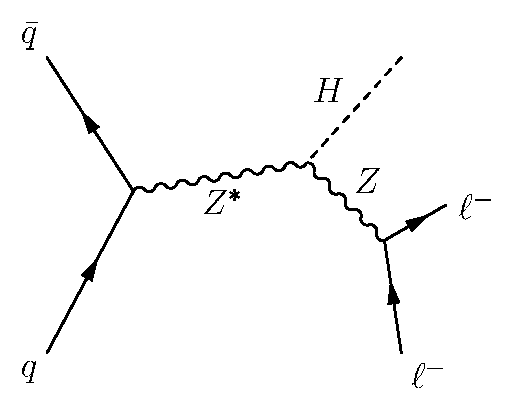
\includegraphics[width=0.8\linewidth]{img/feyn_Zll.pdf} 

\end{block}

\end{columns}

We used recently published results from CMS analysis  HIG-13-018 which reported an upper limits on the invisible branching fraction of a 125 GeV Higgs of 75\%.

\end{frame}

% ###################################################
\begin{frame}{Combination Results}
  
\begin{columns}
 
\column[t]{0.45\linewidth}
\begin{block}{Combined Limits on invisible Higgs}
 
\centering
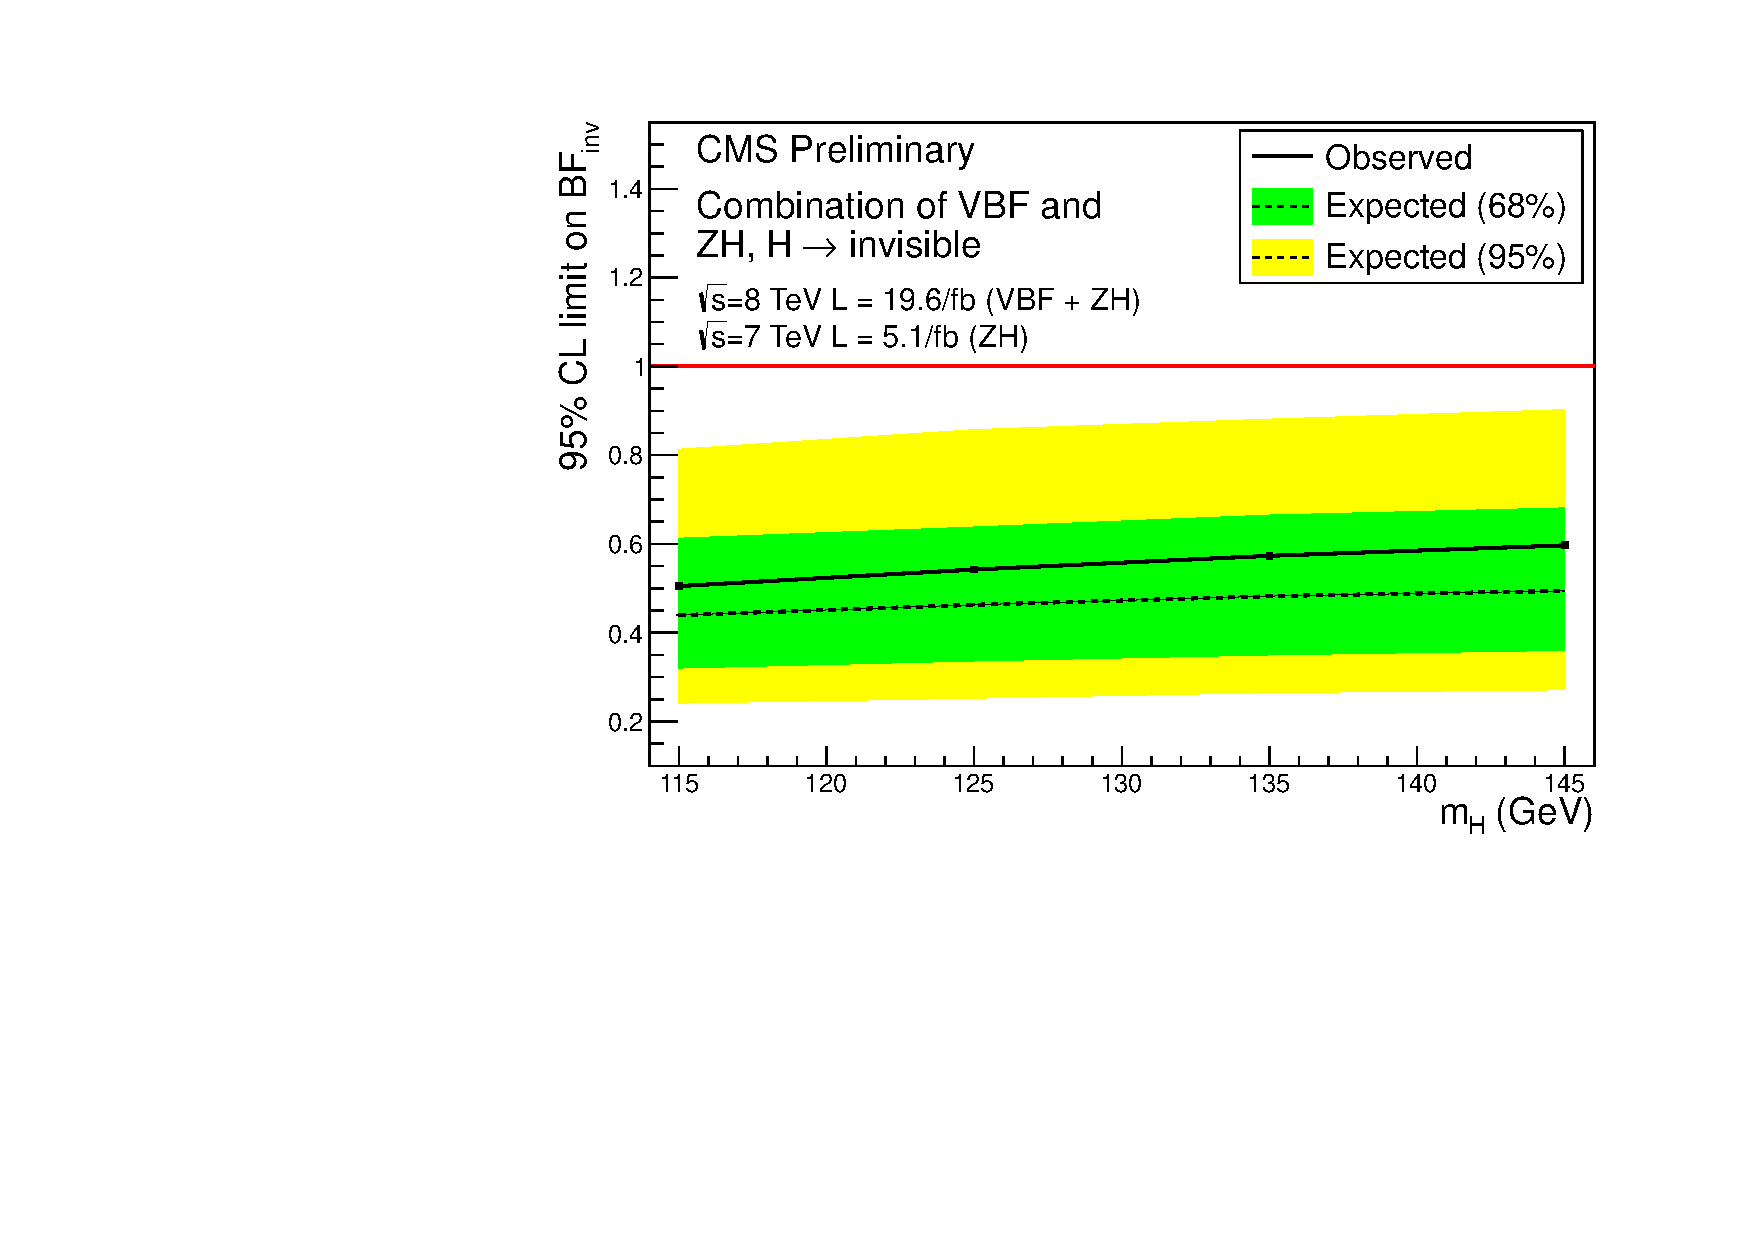
\includegraphics[width=\linewidth]{img/invlimitfinal.pdf} 

\end{block}

\column[t]{0.45\linewidth}
\begin{block}

\begin{itemize}
 \item 95\% CL upper limit on the branching fraction of a Higgs boson to invisible final states as a function of the Higgs boson mass.
 \item SM production cross sections for the Higgs boson have been assumed.
 \item For a Higgs boson of mass 125 GeV the observed (expected) upper limit on the invisible branching fraction is 54 (46)\%.
 \item Systematic errors between analyses are considered uncorrelated.
 \item Combination result including $ZH, (Z \rightarrow b\bar{b})$ are in final stages of approval/publication and takes into account all correlations.
\end{itemize}
 
\end{block}

\end{columns}
 
\end{frame}

% ###################################################
\begin{frame}{Summary}

\begin{block}

\begin{itemize}
 \item A search for an invisibly decaying Higgs boson produced via vector boson fusion has been performed. 
 \item The analysis used a \uline{dedicated trigger and an offline cut} based selection to isolate events with significant \uline{missing energy and two jets} with vector boson fusion characteristics
 \item Major background estimated using data driven methods.  
 \item Using the full $\sqrt{s}=8$ TeV dataset recorded by CMS in 2012, in the signal region:
 \begin{itemize}
  \item Expected background of $339 \pm 36 \stat \pm 50 \syst$ events;
  \item Expected signal of 208 events ($m_H = 125$ BR(Inv.)=100\%);
  \item Observed 390 events in data $\Rightarrow$ \uline{compatible with the expected background} at the 1 $\sigma$ level.
 \end{itemize}
 \item The largest source of uncertainty arises from the statistical uncertainty in the $\Z \rightarrow \mu \mu$ control region. Other important sources of uncertainty:
 \begin{itemize}
  \item V+jets backgrounds MC ratio: 20\% uncertainty
  \item Jet and $\met$ energy scales and resolution for $\Z \rightarrow \nu \nu$ and $\W \rightarrow \ell \nu$: 5-10\% uncertainty
  \item Jet and $\met$ energy scales and resolution for $\W \rightarrow \tau_{\rm had} \nu$: 15\% uncertainty
 \end{itemize} 
 \item Using an asymptotic ${\rm CL}_{\rm S}$ method, 95\% CL upper limits are placed on the production cross section times invisible branching fraction.  The observed limit on the invisible branching fraction of the 125 GeV Higgs is 69\%, with an expected limit of 53\%.  
 \item A combination with $ZH, (Z \rightarrow b\bar{b})$ is presented and the observed (expected) upper limit on the invisible branching fraction is 54 (46)\%
 \item This combination is the \uline{most sensitive} to invisible decays measurement of the Higgs boson to date.
\end{itemize}

\end{block}

\end{frame}

% ###################################################
\appendix
% ###################################################
\begin{frame}
 
\begin{block}

\begin{center}Backup Slides\end{center}

\end{block}

\end{frame}

% ###################################################
\begin{frame}{The CMS Experiment}
 
\begin{block}{Compact Muon Solenoid}

    \begin{columns}
      \column[t]{6.5cm}

      \begin{itemize}
        \item Located at point 5 of the Large Hadron Collider 
        \item General purpose experiment
        \item Objective of studying a broad spectrum of physics
        \item Classical onion structure
        \item One of the most powerful solenoid ever built (3.8 $T$)
      \end{itemize}  

      \column[t]{4.5cm}
      \begin{center}
        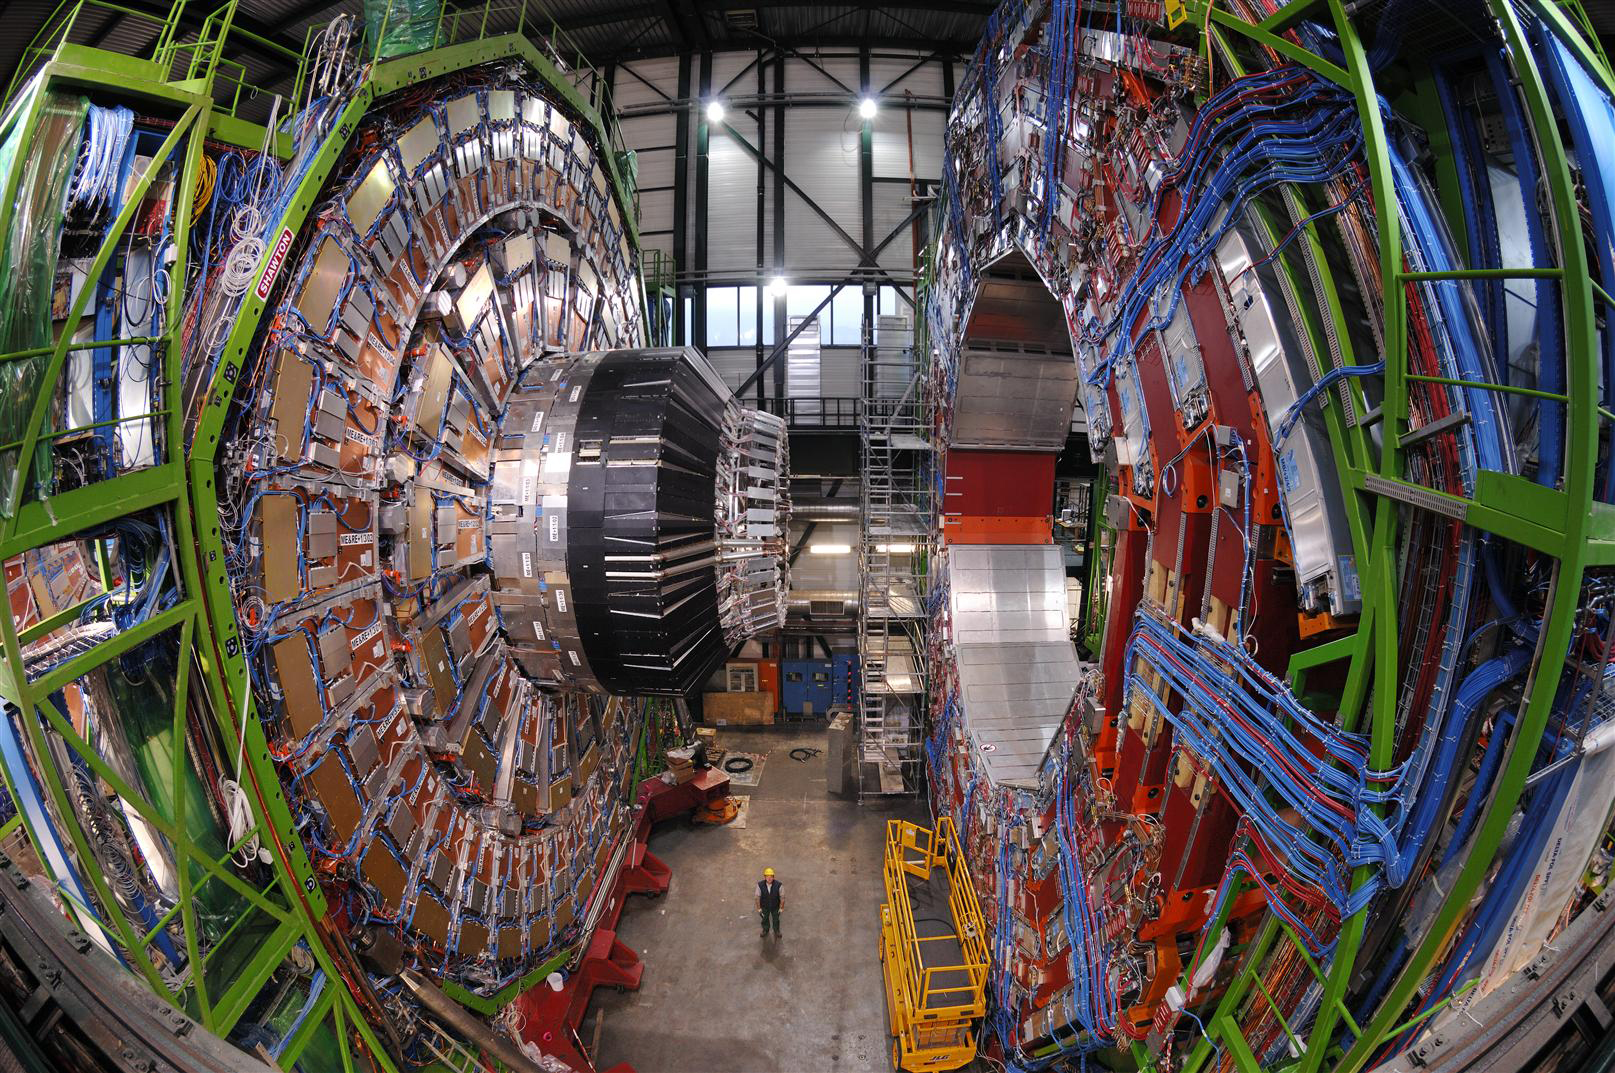
\includegraphics[width=1.00\textwidth]{img/CMSOpen.jpg} 
      \end{center}

    \end{columns}

\end{block}
\begin{block}{CMS strong points for VBF Higgs to invisible search}  

\begin{itemize}
  \item High detector coverage ($\sim4 \pi$)
  \begin{itemize}
    \item Precise measurement of event properties
    \item Accurate missing transverse energy calculation (MET)  
  \end{itemize}
  \item Excellent object position/energy resolution capabilities
  \item Dedicated VBF trigger
  \item This analysis utilises the information from all parts of the detector.
\end{itemize}

\end{block}

\end{frame}

\begin{frame}{Particle Detection on CMS}

When a collision happens then resulting particles need to be identified and measured
 
 \begin{block}{Detector Structure}

  \begin{columns}
    \column[t]{8.0cm}
 
      \begin{center}
        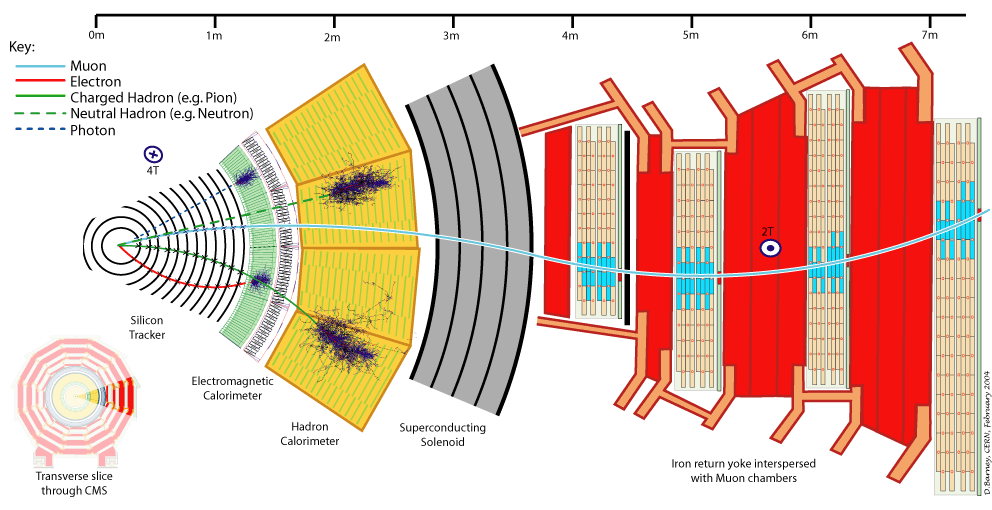
\includegraphics[width=1.00\textwidth]{img/CMS_Slice.png} 
      \end{center}  
      \column[t]{3.5cm}

       \begin{itemize}
         \item Tracker
         \begin{itemize}
           \item Charged particle trajectory
         \end{itemize}
         \item ECAL and HCAL
         \begin{itemize}
           \item Energy Measurement
         \end{itemize}
         \item Solenoid
         \begin{itemize}
           \item Charge and Momentum 
         \end{itemize} 
         \item Muon Chambers
         \begin{itemize}
           \item Muon identification and measurement 
         \end{itemize} 
         \item Trigger (L1+HLT)
         \begin{itemize}
           \item Event Selection 
         \end{itemize} 
       \end{itemize}

    \end{columns}

  \end{block}

  \begin{itemize}
    \item Detector subsystems are designed to take advantage of particle characteristics in order to identify and measure
          their properties.
    \item Trigger System is responsible to select only the most interesting events.
  \end{itemize} 

\end{frame}

\end{document}